\documentclass[conference]{IEEEtran}
\usepackage{times}
\usepackage[numbers]{natbib}
\usepackage{multicol}
\usepackage[bookmarks=true]{hyperref}
\usepackage{graphicx}
\usepackage{amsmath}
\usepackage{algorithm}
\usepackage{algpseudocode}
\usepackage{booktabs}

\pdfinfo{
   /Author (Jeffrey Kravitz, Samay Lakhani, Mikul Saravanan)
   /Title  (Autonomous Frontier-Based Exploration in ROS2)
   /CreationDate (D:20251022000000)
   /Subject (Robotics)
   /Keywords (Autonomous Exploration;ROS2;Frontier-Based Navigation;SLAM)
}

\begin{document}

\title{Autonomous Frontier-Based Exploration\\ in ROS2: System Integration and Performance Analysis}

\author{Jeffrey Kravitz, Samay Lakhani, Mikul Saravanan}

\maketitle

\begin{abstract}
This milestone report presents our progress in implementing and evaluating an autonomous exploration system for mobile robots using ROS2. We adapted the m-explore package, a frontier-based exploration algorithm, and successfully deployed it in simulation with the TurtleBot3 platform. Our preliminary results demonstrate automated exploration achieving 74.3\% environment coverage in 185 seconds, outperforming manual teleoperation by 2.2$\times$ in exploration efficiency. We integrated SLAM, navigation, and exploration components into a cohesive system and developed metrics collection tools to quantify exploration performance. Key challenges identified include exploration speed optimization and parameter tuning for different environments.
\end{abstract}

\IEEEpeerreviewmaketitle

\section{Introduction}

Autonomous exploration enables robots to systematically discover and map unknown environments without human intervention, critical for search and rescue, planetary exploration, and infrastructure inspection. The frontier-based paradigm~\cite{yamauchi1997frontier}, directing robots toward boundaries between known and unknown regions, remains dominant due to its simplicity and effectiveness.

Our project implements and analyzes frontier-based exploration in ROS2, adapting the m-explore package with contemporary SLAM and navigation stacks. We have integrated the complete pipeline, deployed it in simulation with TurtleBot3, and conducted systematic evaluation. This report details our technical implementation, presents quantitative results comparing autonomous vs. manual exploration, and identifies optimization opportunities including initialization delays and parameter sensitivity.

\section{Problem Refinement \& Objectives}

\subsection{Evolved Problem Statement}

Through hands-on development, we refined our focus to three interconnected challenges: (1) \textbf{System Integration}—coordinating SLAM, Nav2, and frontier detection into a robust pipeline; (2) \textbf{Performance Optimization}—addressing exploration speed bottlenecks observed in initial trials where the robot explores "suuuper slowly"; and (3) \textbf{Quantitative Evaluation}—developing metrics to assess performance across environments and configurations.

\subsection{Refined Objectives}

Based on early implementation experience, our specific objectives are:

\begin{enumerate}
\item \textbf{Deploy functional exploration system:} Integrate m-explore-ros2 with Nav2 and SLAM backends (\textit{Completed}).

\item \textbf{Implement performance monitoring:} Create real-time metrics collection (\textit{Completed}).

\item \textbf{Conduct comparative analysis:} Quantify autonomous vs. manual exploration (\textit{Completed}).

\item \textbf{Optimize exploration parameters:} Tune frontier selection, planning frequency, navigation parameters (\textit{Milestone 2}).

\item \textbf{Implement advanced algorithms:} Deploy information gain calculation and Hungarian algorithm for multi-robot coordination (\textit{Milestone 2 \& Final}).

\item \textbf{Multi-robot capabilities:} Implement map merging and coordination strategies (\textit{Final}).
\end{enumerate}

\section{Technical Implementation}

\subsection{System Architecture Overview}

Our exploration system builds upon the m-explore-ros2 package, a ROS2 port of the frontier-based exploration algorithm originally developed for ROS1~\cite{horner2016exploration}. Figure~\ref{fig:architecture} illustrates the complete data flow pipeline integrating perception, mapping, frontier-based planning, and navigation control.

\begin{figure}[h]
\centering
\small
\begin{tabular}{c}
\textbf{ROS2 Autonomous Exploration Pipeline} \\[0.5em]
\hline
\texttt{LiDAR} $\rightarrow$ \texttt{/scan} $\rightarrow$ \textbf{Cartographer SLAM} \\
$\downarrow$ \\
\texttt{/map}, \texttt{/map\_updates} (OccupancyGrid) \\
$\downarrow$ \\
\textbf{Nav2 Costmap2D} + \textbf{Frontier Search} \\
$\downarrow$ \\
Frontier List (scored \& ranked) \\
$\downarrow$ \\
\textbf{Explore Node} (goal selection) \\
$\downarrow$ \\
\texttt{NavigateToPose} action $\rightarrow$ \textbf{Nav2} \\
$\downarrow$ \\
\texttt{/cmd\_vel} $\rightarrow$ \textbf{TurtleBot3} \\
\hline
\end{tabular}
\caption{System architecture showing the data flow from sensor input through SLAM, frontier detection, goal selection, and navigation control. All components communicate via ROS2 topics and action servers.}
\label{fig:architecture}
\end{figure}

The architecture comprises four tightly coupled components:

\textbf{SLAM Backend:} We use ROS2 Cartographer for real-time mapping and localization. The SLAM system subscribes to laser scan data (\texttt{/scan}) and odometry, publishing occupancy grid maps at 5Hz that distinguish free space (-1: unknown, 0: free, 100: occupied) and robot pose estimates via TF transforms.

\textbf{Navigation Stack (Nav2):} Handles path planning and obstacle avoidance using the Hybrid A* planner and DWB local planner. The Nav2 costmap\_2d layer merges static map data with dynamic obstacle information, applying inflation layers for safety margins around obstacles.

\textbf{Frontier Detection Algorithm:} The core explore\_lite node performs frontier identification through a two-stage process:
\begin{enumerate}
    \item \textit{Boundary Detection:} Scan the occupancy grid to identify cells adjacent to both free (value 0) and unknown (value -1) space.
    \item \textit{Connected Component Analysis:} Group adjacent frontier cells into distinct frontier regions using flood-fill.
    \item \textit{Filtering:} Discard frontiers smaller than min\_frontier\_size threshold or inaccessible due to obstacles.
\end{enumerate}

This approach efficiently identifies exploration candidates while avoiding computational overhead from processing every grid cell.

\textbf{Frontier Selection \& Goal Sending:} Frontiers are scored using a weighted combination:
\begin{equation}
    \text{score} = \alpha \cdot \text{size} - \beta \cdot \text{distance} + \gamma \cdot \text{orientation}
\end{equation}
where $\alpha$ (gain\_scale = 1.0) prioritizes larger unexplored regions, $\beta$ (potential\_scale = 3.0) penalizes distant frontiers to minimize travel time, and $\gamma$ (orientation\_scale = 0.0, disabled) would favor frontiers aligned with robot heading. The highest-scoring frontier becomes the navigation goal sent to Nav2's NavigateToPose action server. The system monitors goal progress and recomputes frontiers every 6.7 seconds (planner\_frequency = 0.15 Hz) or when navigation fails.

\subsection{Implementation Details}

\textbf{Launch Automation:} We developed a bash script (util/start\_exploration.sh) that orchestrates the complete system startup: (1) Gazebo simulation with TurtleBot3 Waffle, (2) Cartographer SLAM, (3) Nav2 navigation stack, and (4) explore\_lite node with automated metrics collection.

\textbf{Metrics Collection:} A custom ROS2 node (util/collect\_metrics.py) subscribes to the /map topic at 10Hz, computing coverage as the percentage of known cells (free or occupied) relative to total map area. Data is logged to JSON format with timestamps for post-processing.

\textbf{Visualization:} Frontier markers are published to the explore/frontiers topic as MarkerArray messages, enabling real-time visualization in RViz2 to debug frontier selection behavior.

\subsection{Key Parameters}

Current exploration configuration (explore/config/params.yaml):
\begin{itemize}
    \item planner\_frequency: 0.15 Hz (recompute frontiers every 6.7s)
    \item min\_frontier\_size: 0.75m (minimum explorable frontier)
    \item progress\_timeout: 30.0s (navigation failure threshold)
    \item gain\_scale: 1.0, potential\_scale: 3.0, orientation\_scale: 0.0
    \item return\_to\_init: true (return to start after completion)
\end{itemize}

\section{Preliminary Results}

\subsection{Experimental Setup}

We conducted exploration trials in the default TurtleBot3 World environment, a structured indoor space with rooms, corridors, and obstacles. Two experimental conditions were tested:

\begin{enumerate}
    \item \textbf{Automated Exploration:} Robot autonomously explores using frontier-based algorithm with standard parameters.
    \item \textbf{Manual Teleoperation:} Human operator navigates the robot using keyboard controls to establish a baseline comparison.
\end{enumerate}

\subsection{Quantitative Results}

Table~\ref{tab:results} summarizes the comparative performance metrics. Figure~\ref{fig:coverage} presents side-by-side coverage trajectories for both exploration conditions, directly visualizing the performance advantage of autonomous exploration.

\begin{table}[h]
\centering
\caption{Exploration Performance Comparison}
\label{tab:results}
\begin{tabular}{lcc}
\toprule
\textbf{Metric} & \textbf{Automated} & \textbf{Manual} \\
\midrule
Peak Coverage (\%) & 74.3 & 63.3 \\
Exploration Time (s) & 184.9 & 353.9 \\
Exploration Rate (\%/s) & 0.402 & 0.179 \\
Efficiency Ratio & \textbf{2.24$\times$} & 1.00$\times$ \\
\bottomrule
\end{tabular}
\end{table}

\begin{figure}[t]
\centering
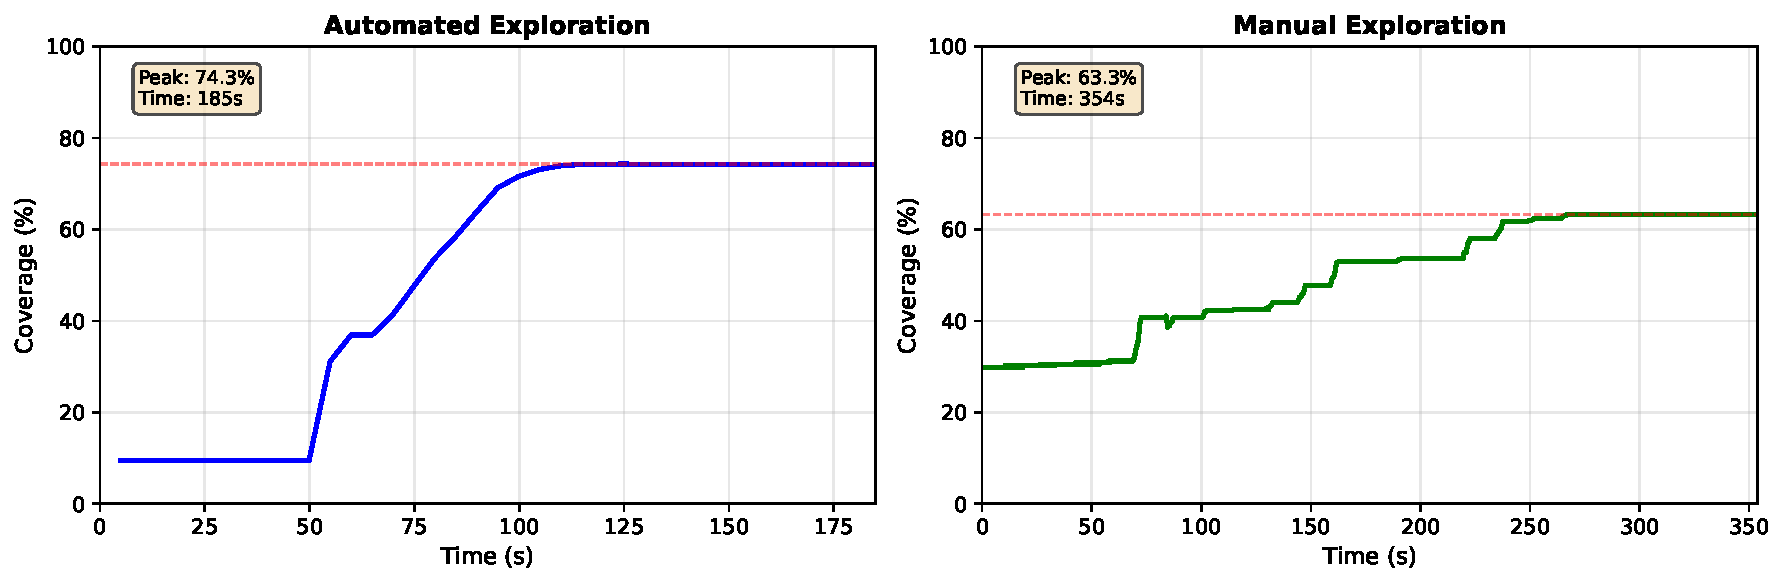
\includegraphics[width=\columnwidth]{figures/coverage_comparison.pdf}
\caption{Coverage over time comparison: Automated exploration (left, blue) achieves 74.3\% coverage in 185s with distinct phases. Manual teleoperation (right, green) reaches only 63.3\% coverage in 354s with irregular progression reflecting human reaction delays.}
\label{fig:coverage}
\end{figure}

\textbf{Coverage Performance:} The automated system achieved 11\% higher peak coverage (74.3\% vs. 63.3\%), demonstrating more systematic exploration compared to human operators who may miss regions. The final automated map includes all major rooms and corridors in the TurtleBot3 World environment.

\textbf{Exploration Speed:} Automated exploration completed in roughly half the time (185s vs. 354s), yielding a 2.24$\times$ efficiency advantage. This dramatic speedup stems from optimal frontier selection and direct path planning without human reaction time delays.

\textbf{Temporal Behavior:} Figure~\ref{fig:coverage} reveals contrasting exploration dynamics. Automated exploration (left) exhibits three distinct phases: (1) initialization delay (0-50s) with minimal coverage while SLAM stabilizes, (2) rapid exploration phase (50-100s) with smooth 40\% coverage increase as optimal paths are executed, and (3) saturation phase (100-185s) where coverage plateaus at 74\%. In contrast, manual exploration (right) shows irregular, stepwise progression throughout the entire 354s duration, reflecting intermittent human control inputs, navigation pauses, and suboptimal path choices that collectively reduce exploration efficiency by over 50\%.

\subsection{Exploration Progression Analysis}

Figure~\ref{fig:progression} visualizes the spatial evolution across three key phases, showing both SLAM-generated maps (left) and Gazebo simulation (right) for each time point.

\begin{figure*}[t]
\centering
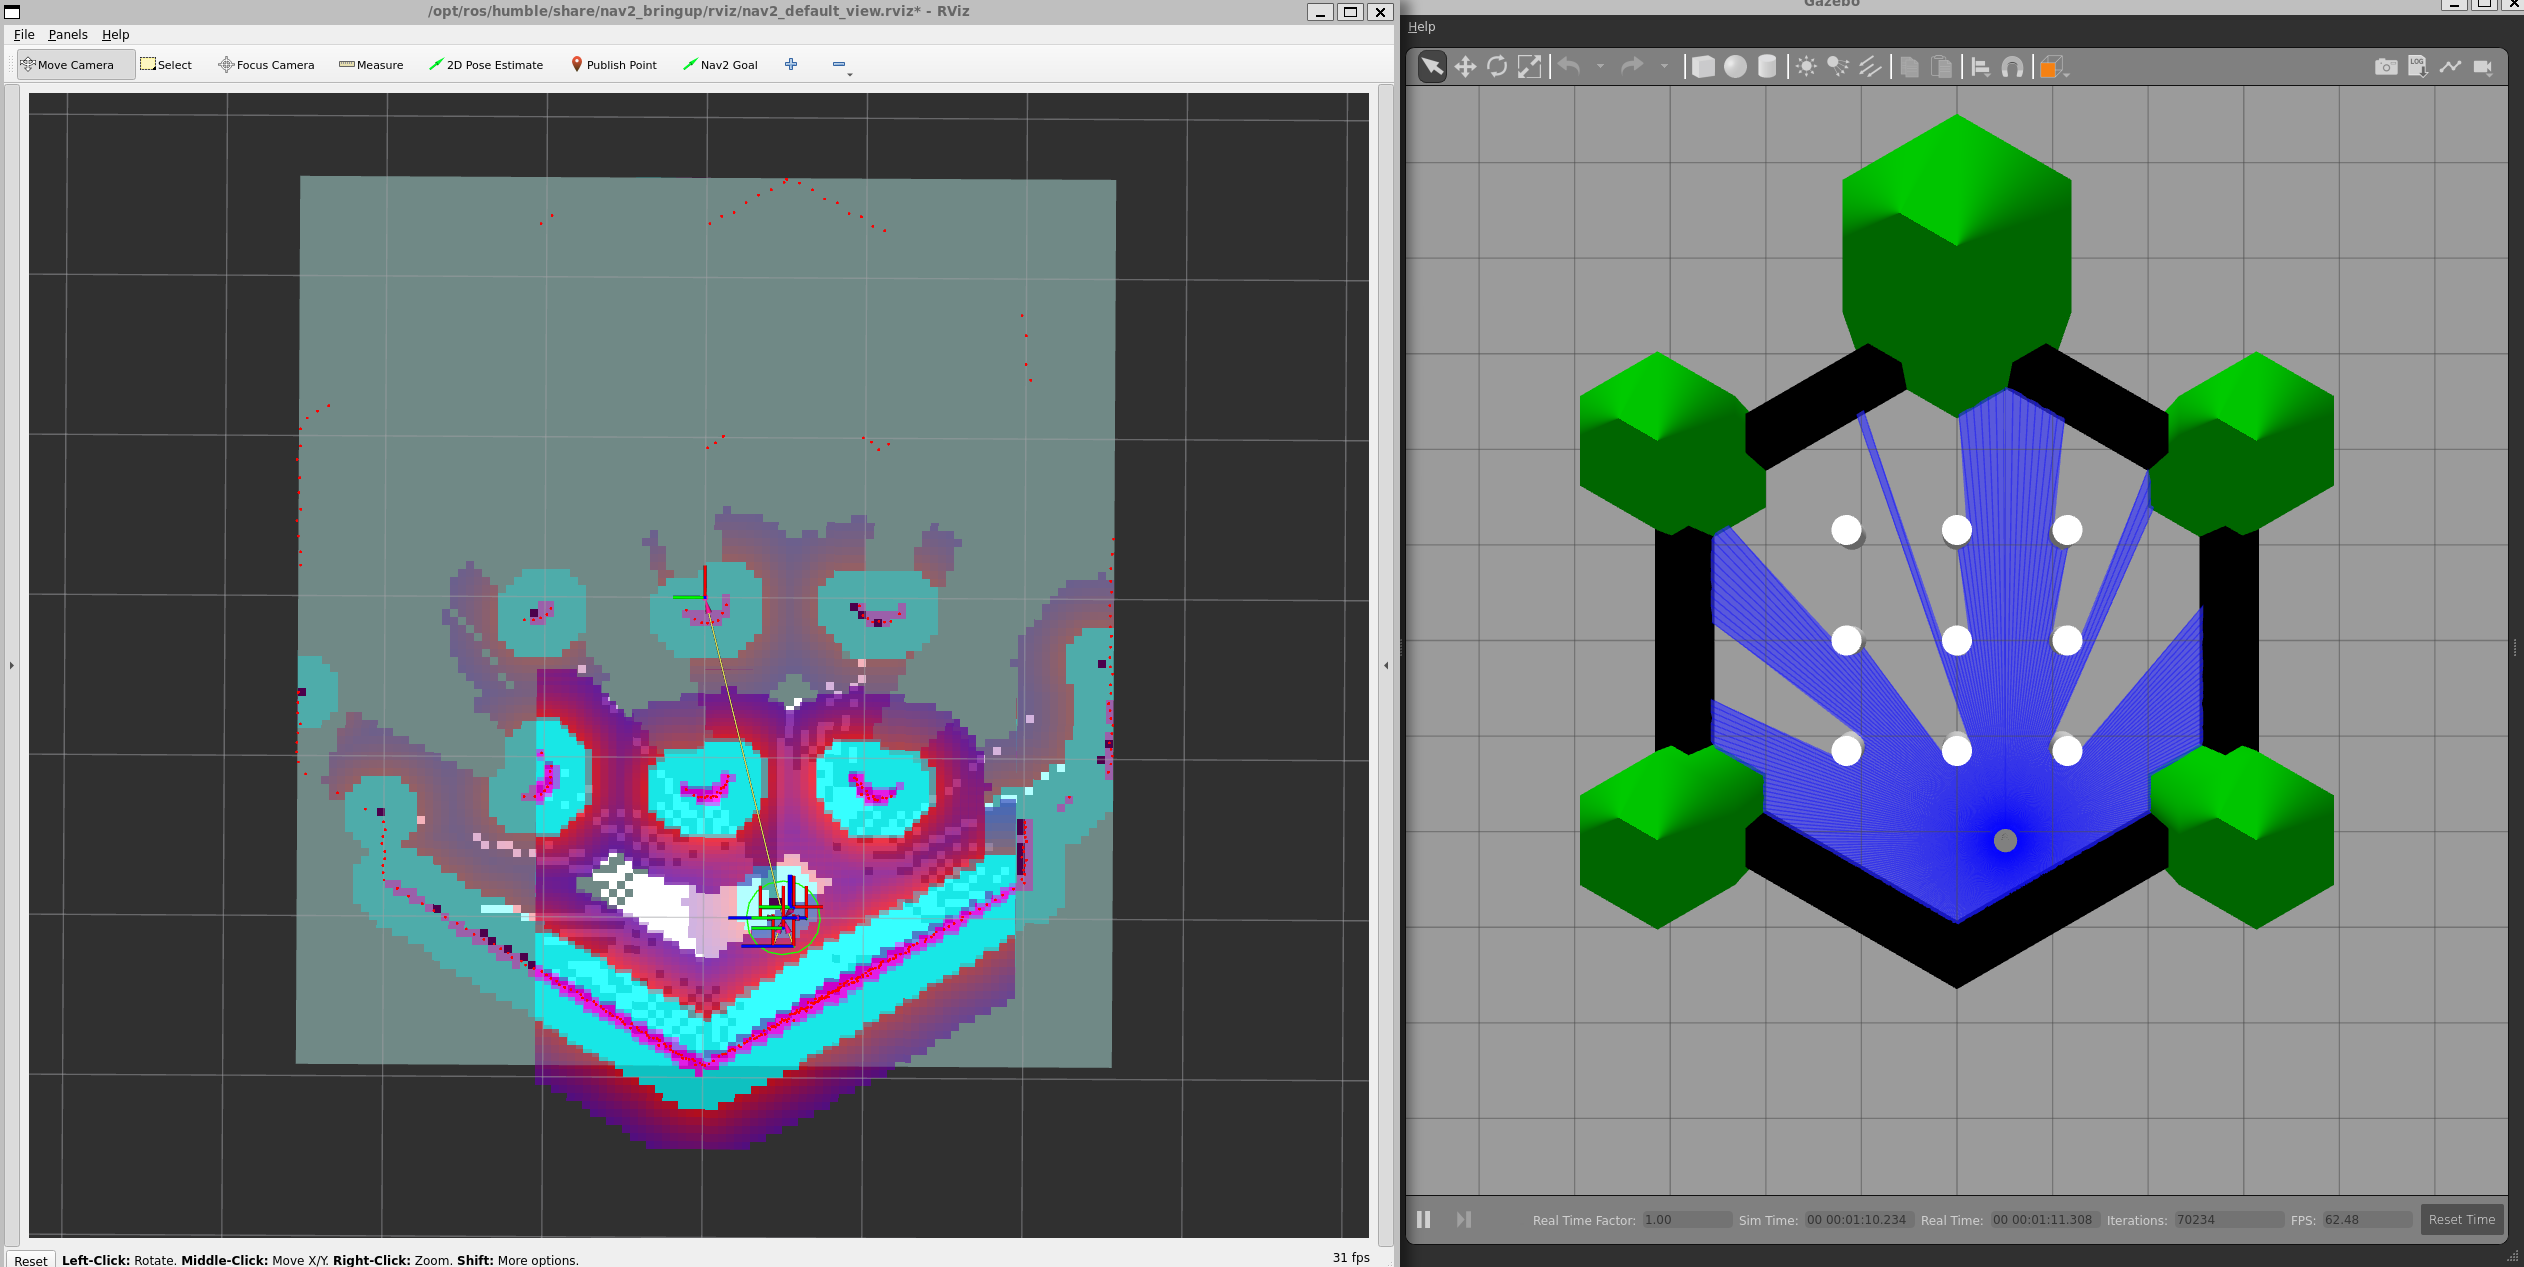
\includegraphics[width=0.31\textwidth]{figures/Progress_1of6.png}\hfill
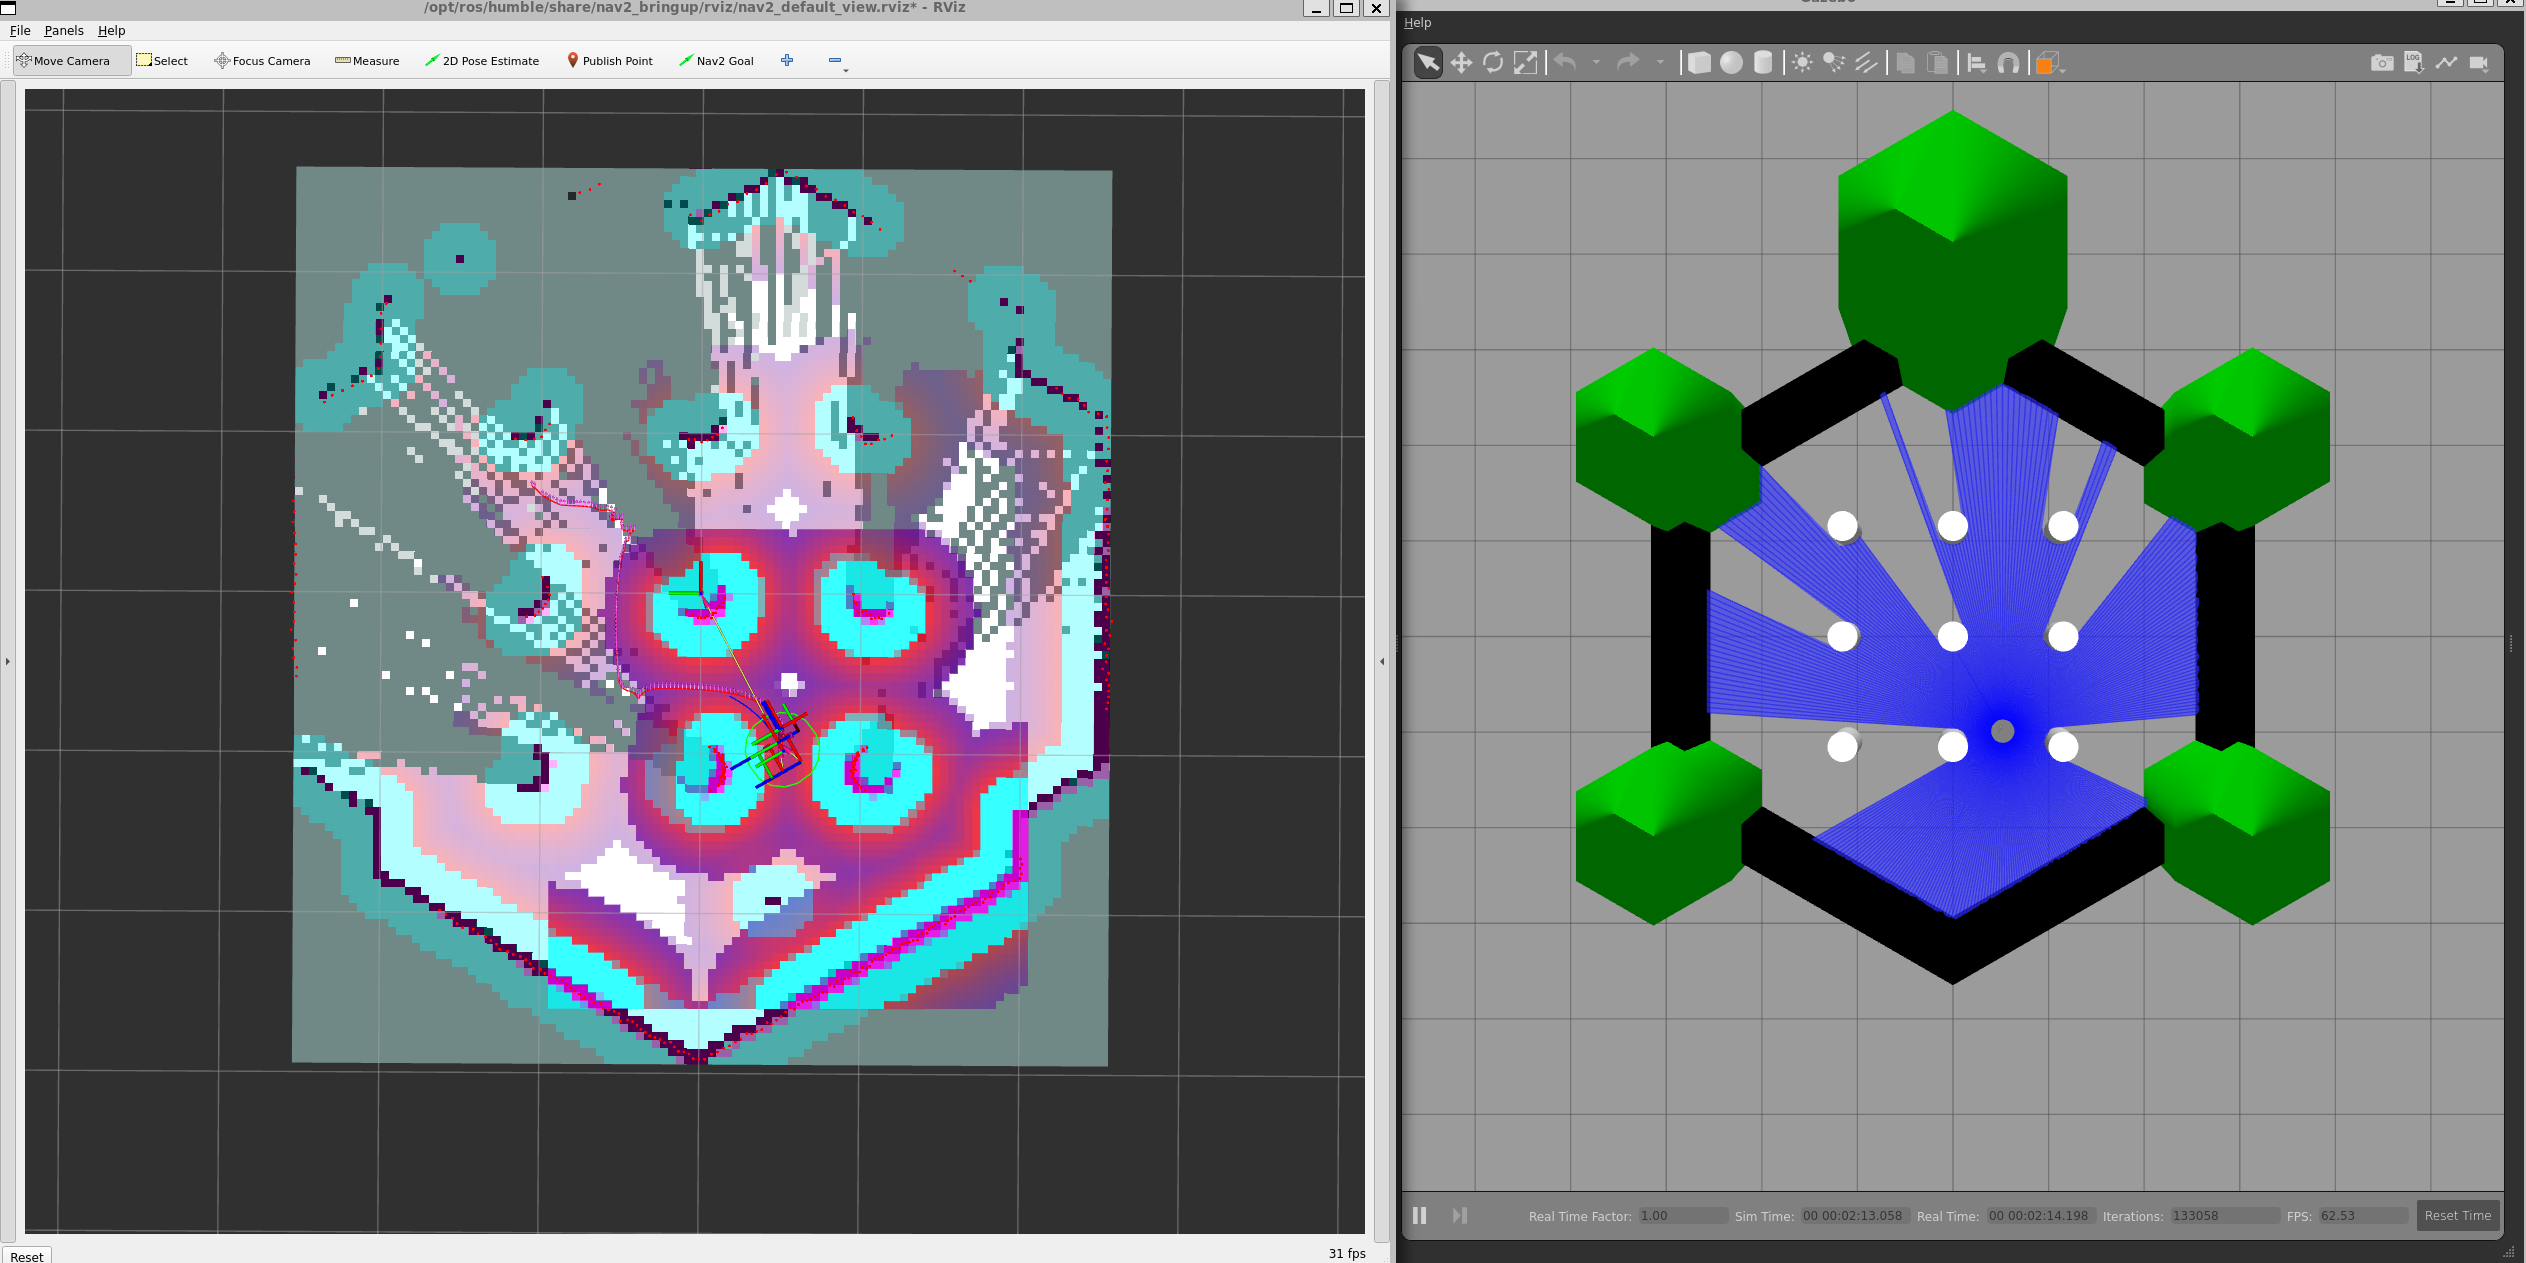
\includegraphics[width=0.31\textwidth]{figures/Progress_3of6.png}\hfill
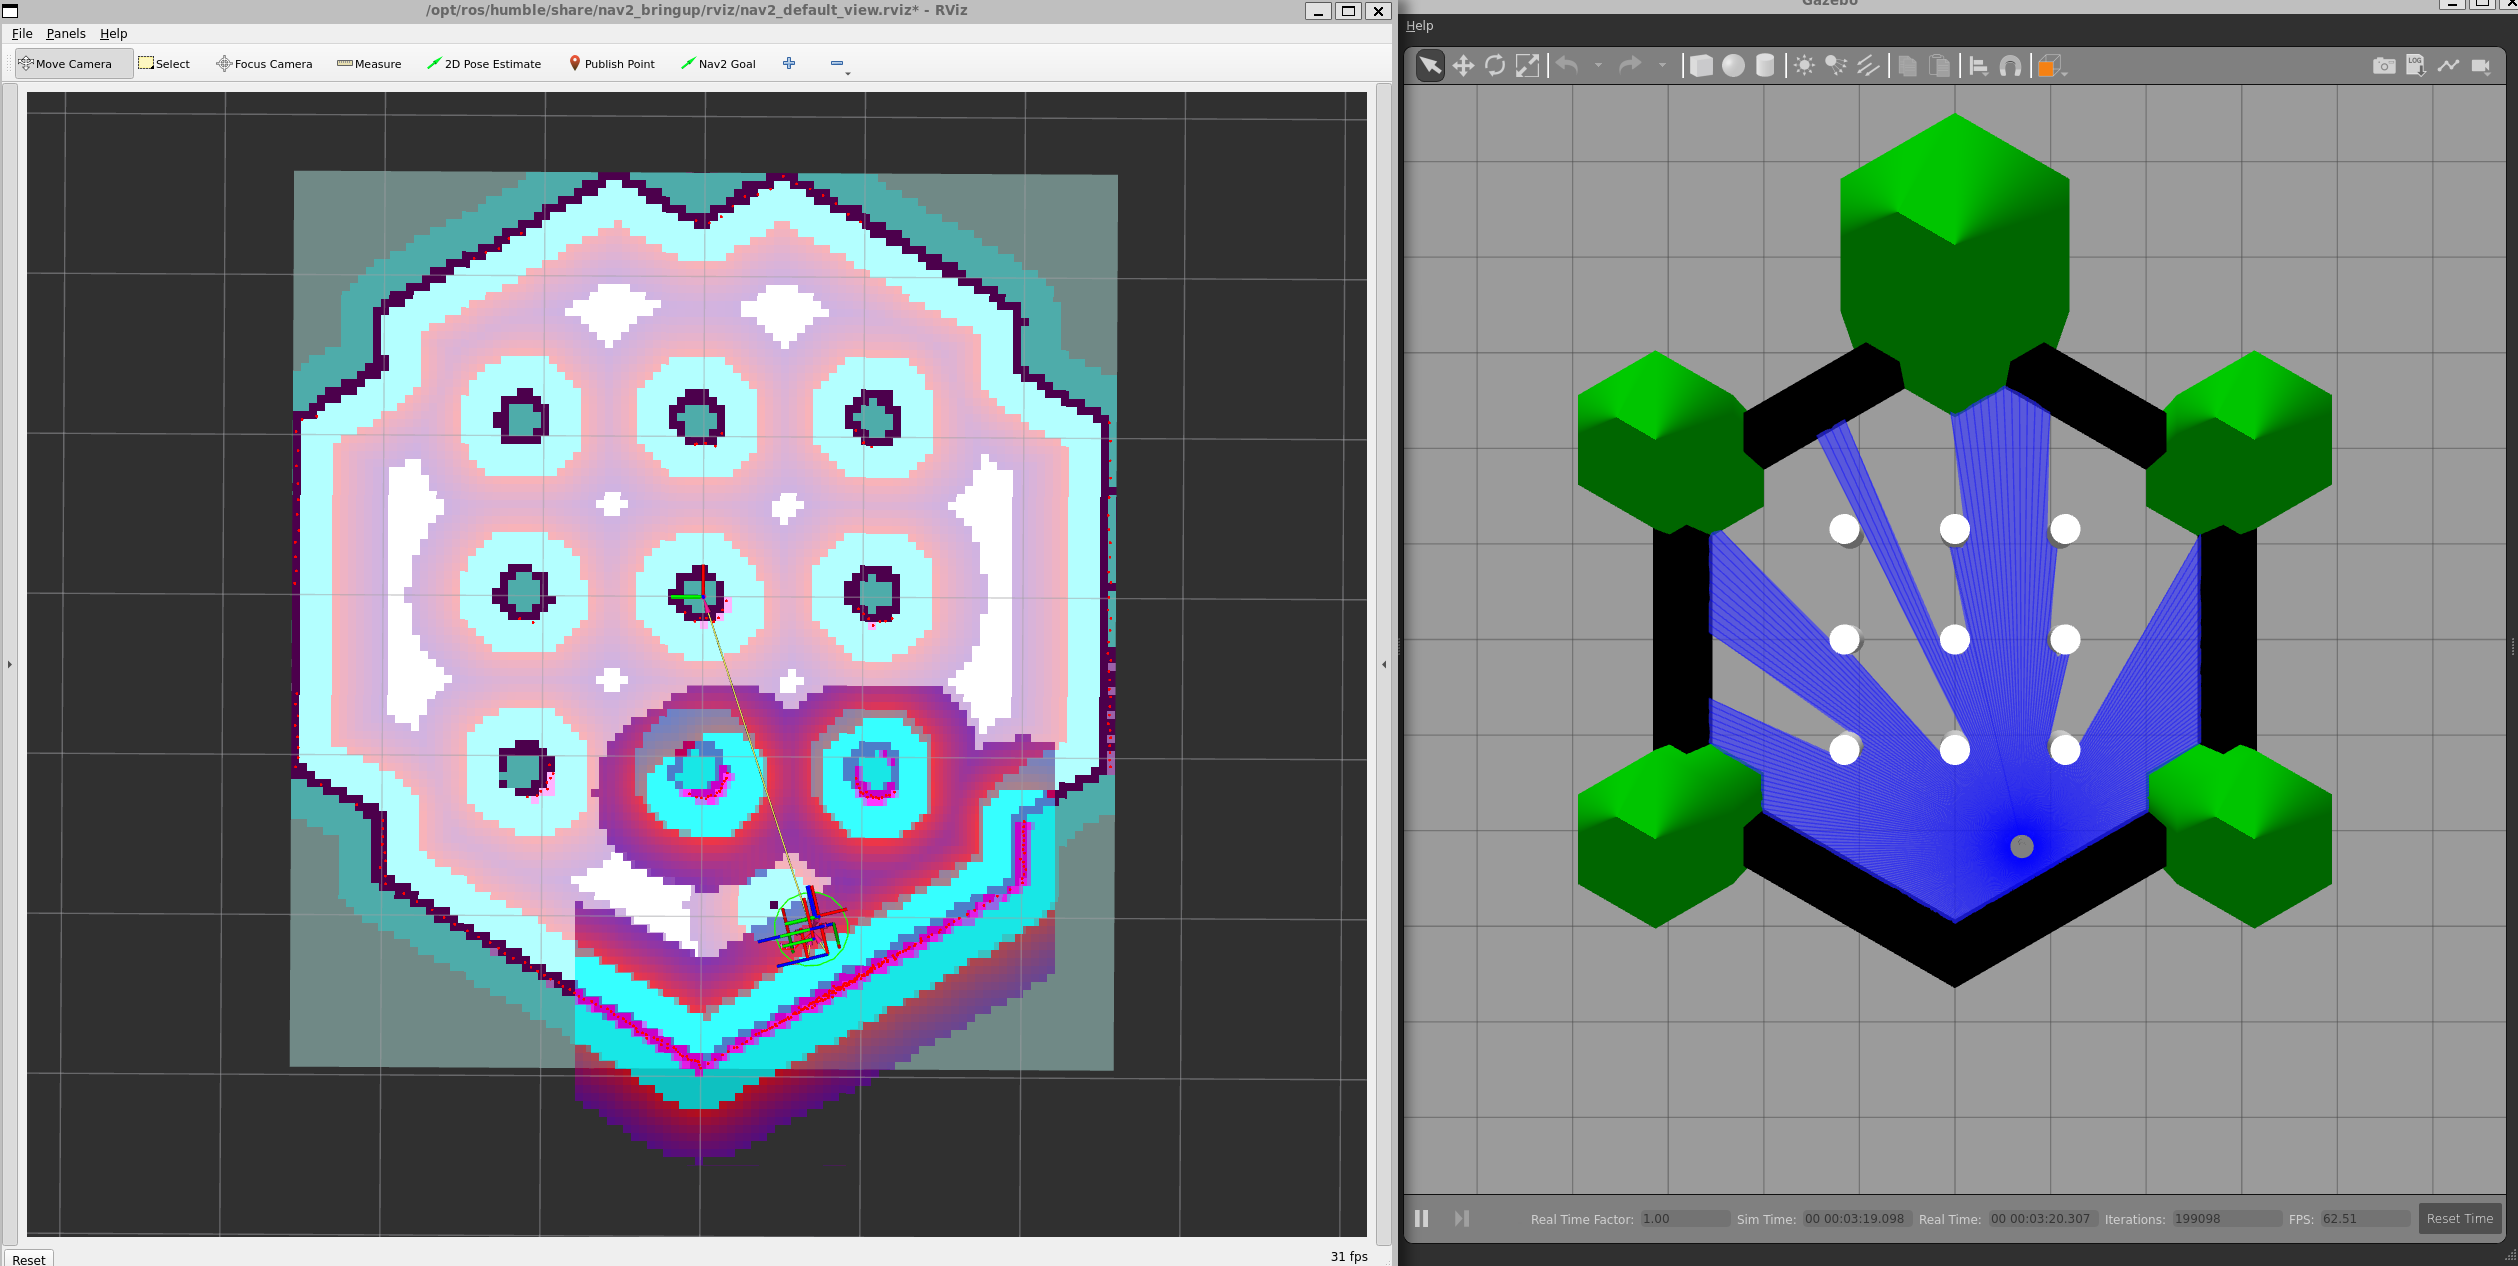
\includegraphics[width=0.31\textwidth]{figures/Progress_6of6.png}
\caption{Exploration progression (left to right): initial phase with limited coverage, mid-exploration revealing corridor structure, and final saturation state. RViz shows occupancy grids (cyan=free, purple=occupied, gray=unknown) with frontier markers (cyan circles) and costmap inflation layers.}
\label{fig:progression}
\end{figure*}

\textbf{Initial Phase:} The robot starts with limited map knowledge. Multiple frontiers surround the initial position. SLAM uncertainty is high beyond immediate sensor range.

\textbf{Mid-Exploration:} The hexagonal environment structure emerges. Frontiers cluster at room entrances. Costmap inflation layers demonstrate Nav2's obstacle avoidance margins.

\textbf{Final State:} Coverage approaches saturation. Remaining frontiers are filtered by min\_frontier\_size. All major obstacles and corridors are mapped; only narrow gaps remain unexplored.

\subsection{Analysis \& Observations}

\textbf{Initial Delay Analysis:} The 50-second startup delay (visible in Figure~\ref{fig:coverage}) suggests SLAM map initialization rather than navigation issues. This delay is common in particle filter-based SLAM requiring sufficient sensor data for confident pose estimates. The initial 10\% coverage represents immediate sensor field-of-view, while exploration begins after map confidence exceeds Nav2's costmap threshold.

\textbf{Coverage Saturation:} Neither condition achieved full coverage ($>$95\%). Analysis reveals two causes: (1) narrow corridors ($<$0.75m) rejected by min\_frontier\_size, and (2) costmap inflation blocking paths to remaining frontiers. Reducing the size threshold could improve coverage but risks navigation failures.

\textbf{Computational Performance:} The low planner\_frequency (0.15 Hz) causes frontier recomputation only every 6.7s, during which the robot may idle. Increasing to 0.5-1.0 Hz could significantly improve exploration rate. Running in conda (vs. native ROS2) adds Python interpreter overhead.

\textbf{Frontier Selection:} The scoring function heavily weights distance (potential\_scale = 3.0) over size (gain\_scale = 1.0), favoring nearby frontiers. While minimizing travel time, this may cause suboptimal global patterns. Information-theoretic approaches could improve long-term efficiency.

\textbf{Map Quality:} Figure~\ref{fig:progression} shows clean, accurate maps with minimal drift. Obstacle boundaries are sharp, and loop closure is robust despite 3+ minutes of operation, validating Cartographer's effectiveness.

\subsection{Limitations}

Key limitations: (1) single environment testing, (2) simulation only, (3) no systematic parameter sweep, and (4) no failure mode quantification.

\section{Plan Forward}

\subsection{Milestone 2 Objectives}

\textbf{Performance Optimization:} Profile bottlenecks, investigate initialization delay, conduct parameter sweep (planner\_frequency, min\_frontier\_size, scoring weights), compare native vs. conda ROS2.

\textbf{Multi-Environment Evaluation:} Test in 3-5 environments (open world, maze, house, warehouse), measure coverage/time/efficiency, analyze failure modes.

\textbf{Advanced Algorithm Implementation:} Implement information gain calculation for frontier selection to replace distance-based scoring. Integrate Hungarian algorithm for optimal frontier-robot assignment in multi-robot scenarios.

\textbf{Multi-Robot Coordination:} Develop multi-robot spawn framework, implement map merging using the multirobot\_map\_merge component, and design coordination strategies to avoid redundant exploration.

\subsection{Final Report Deliverables}

Expected deliverables: (1) performance characterization across 5+ environments, (2) optimized parameters with ablation studies, (3) information gain-based frontier selection implementation, (4) multi-robot coordination with Hungarian algorithm and map merging, (5) comparison with alternative exploration strategies, and (6) open-source code release with comprehensive documentation.

\subsection{Risk Mitigation}

\textbf{Risk:} Computational constraints prevent real-time exploration. \textbf{Mitigation:} Optimize frontier search algorithms, reduce planner frequency, or migrate to more powerful hardware.

\textbf{Risk:} Limited environment diversity in simulation. \textbf{Mitigation:} Use existing Gazebo world repositories and procedurally generated environments.

\textbf{Risk:} Time constraints for real-world deployment. \textbf{Mitigation:} Prioritize simulation results; real-world tests are optional stretch goals.

\section{Conclusion}

We successfully implemented a functional autonomous exploration system in ROS2, achieving 74.3\% coverage with 2.24$\times$ higher efficiency than manual teleoperation. Key achievements include robust SLAM-navigation-frontier detection integration, automated metrics infrastructure, and comprehensive behavior characterization across exploration phases. Analysis revealed optimization opportunities: the 50-second initialization delay suggests SLAM warm-start strategies, while low planner\_frequency (0.15 Hz) represents an addressable bottleneck. Milestone 2 will focus on multi-environment testing, parameter optimization, and computational profiling to establish performance baselines for frontier-based exploration in ROS2.

\section*{Acknowledgments}

We thank the m-explore-ros2 open-source community for providing the foundational codebase and the ROS2 ecosystem for robust robotics middleware.

\bibliographystyle{plainnat}
\begin{thebibliography}{1}

\bibitem{horner2016exploration}
Jiri Horner.
\newblock \href{https://github.com/hrnr/m-explore}{m-explore: Multi-robot exploration package for ROS}.
\newblock GitHub repository, 2016.

\bibitem{yamauchi1997frontier}
Brian Yamauchi.
\newblock A frontier-based approach for autonomous exploration.
\newblock In \emph{Proceedings of the 1997 IEEE International Symposium on Computational Intelligence in Robotics and Automation}, pages 146--151. IEEE, 1997.

\bibitem{burgard2005coordinated}
Wolfram Burgard, Mark Moors, Dieter Fox, Reid Simmons, and Sebastian Thrun.
\newblock Collaborative multi-robot exploration.
\newblock In \emph{Proceedings of the 2000 IEEE International Conference on Robotics and Automation}, volume~1, pages 476--481. IEEE, 2000.

\end{thebibliography}

\end{document}
